% ---------------------------------------------------------------------
% Das Dokument kompiliert mit pdflatex und ist auf Basis 
% von Koma-Script entstanden. 
%
% Autor des Templates (für Anmerkungen): 
% Michael von Riegen, riegen@informatik.uni-hamburg.de
%
% Einzelne Code-Teile für das Titelblatt sind aus dem Template 
% von Benjamin Kirchheim entnommen.
% Neue Titelseite von Josef Holnburger
%
% 25.05.09, Frank Langanke: Vorlage auf aktuelle KOMA-Version aktualisiert
% 26.05.09, Michael von Riegen: Anmerkung --> aktuelles Koma-Script ist nötig!
% 17.10.2016 neues Uni logo
% 21.08.2018 biblatex und scrlayer-scrpage statt scrpage2, anpassen auf SoWi-Layout
% ---------------------------------------------------------------------

% Wir nutzen Biblatex und biber für das Literaturverzeichnis
\documentclass[12pt, twoside=false, bibliography=totoc, numbers=endperiod, headings=normal, toc=chapterentrydotfill]{scrbook}
\usepackage[backend=biber, style=authoryear-ibid, eprint=false, url=false, doi=false,isbn=false]{biblatex}
\addbibresource{Bib.bib}

% Daten der Hausarbeit
\newcommand\myTitle{Geschlechterunterschiede in den Reden des Deutschen Bundestages}
\newcommand\mySubTitle{Auswertung des 19. Deutschen Bundestages}
\newcommand\thesisType{Projektarbeit}
\newcommand\dateOfSubmission{XX.XX.XXXX}

% Import von Paketen und Optionen die das gesamte Dokument betreffen
% sind in myPreamble.sty ausgelagert.
\usepackage{myPreamble}

\begin{document}


% TITELSEITE
% *************************************************************************
% *    Thesis / Dissertation Latex Template                                        
% *    
% *    Author: Leonard Heilig <leonard.heilig@uni-hamburg.de>
% *    modified by: Josef Holnburger <josef@holnburger.com>
% *   
% *    Note: some parts of this template are based on the VSIS template
% *              of Michael von Riegen <riegen@informatik.uni-hamburg.de>
% *   
% *************************************************************************

\begin{titlepage}

% START PAGE: -1
\setcounter{page}{-1}    

\begin{minipage}[t]{0.6\textwidth}
\setstretch{1.0}
\flushleft 
			Universität Hamburg \\
			Fachbereich: Sozialwissenschaften \\
			Fachgebiet: Politikwissenschaft \\
			Seminar: Forschungsseminar Vergleichende und Regionalstudien \\ 
			Dozenten: Prof. Kai-Uwe Schnapp \\
			PD Dr. Falk Daviter \\
			Wintersemester 2018/19 \\
\end{minipage}
\hfill
\begin{minipage}[t][1.7cm][b]{0.35\textwidth}
\noindent
\includegraphics[width=\textwidth]{images/UHH-Logo_2010_Farbe_CMYK.pdf}
\end{minipage}

\vspace*{\fill}
\begin{center}
	% THESIS TYPE
	\vspace{1cm}\noindent {\textbf{\thesisType}} \vspace{0.2cm} \\
	% THESIS TITLE
	\textbf{\Large \myTitle} \\
	\textbf{\mySubTitle} \\
	\dateOfSubmission \\
\end{center}
\vspace*{\fill}

\begin{minipage}[t]{0.48\textwidth}
\setstretch{1.0}
    \flushleft 
    Gina-Gabriela Görner \\
    Matrikelnummer: XXX \\
    XXX \vspace{0.1cm} \\ 
	XXX \vspace{0.1cm}  \\
	E-Mail: XXX \\ 
\end{minipage}
\begin{minipage}[t]{0.48\textwidth}
	\flushleft
	\setstretch{1.0}
	Josef Holnburger \\
	Matrikelnummer: XXX \\
	XXX \vspace{0.1cm} \\
	XXX \vspace{0.1cm} \\
	E-Mail: josef@holnburger.com \\
\end{minipage}


\end{titlepage}



% VERZEICHNISSE (Inhaltsverzeichnis, Abkürzungen)
% Vorspann einleiten --> Seitennummerierung römisch
\frontmatter

% Inhaltsverzeichnis
\tableofcontents

% Abbildungs- und Tabllenverzeichnis auf einer Seite
\listoffigures
\addcontentsline{toc}{chapter}{\listfigurename}
\vspace*{24pt}
{\let\clearpage\relax \listoftables}	
\addcontentsline{toc}{chapter}{\listtablename}

% Hauptteil einleiten --> Seitennummerierung wieder arabisch
\mainmatter

\chapter{Einleitung}\label{Einleitung} %Das Label erscheint in den Überschriften der Seiten.

Hier ist ein Beispiel mit einer Quelle und Seitenzahl \parencite[S. 103]{wangnerud_2009}. Hier ist ein Beispiel von \textcite{erikson_2018} mit einem Verweis im Text. Wenn ein Autor in einem Absatz öfter zitiert wird, wird daraus ein ebd. \parencite{erikson_2018}.

Hier eine Tabelle, welche im Ordner \enquote{table} abgespeichert wurde und mit folgendem Befehl eingelesen werden kann. Verweise siehe Tabelle \ref{table:unterbrechung_stats}. Außerdem möchte ich hier noch auf die Abbildung \ref{fig:lda_example} auf Seite \pageref{fig:lda_example} verweisen. 

\begin{table}[htb]
    \centering
    \caption{Statistiken zu Unterbrechungen in den Bundestagsreden}
    
\begin{tabular}{lrrrrrr}
\toprule
Geschlecht & min & max & mean & sd & n & var\\
\midrule
männlich & 0 & 41 & 3.96 & 4.86 & 4173 & 23.60\\
weiblich & 0 & 39 & 3.28 & 4.11 & 1851 & 16.89\\
\bottomrule
\end{tabular}
    \label{table:unterbrechung_stats}
\end{table}

\Blindtext

\section{Unterkapitel}

\blindtext
\\

\begin{figure}
    \centering
    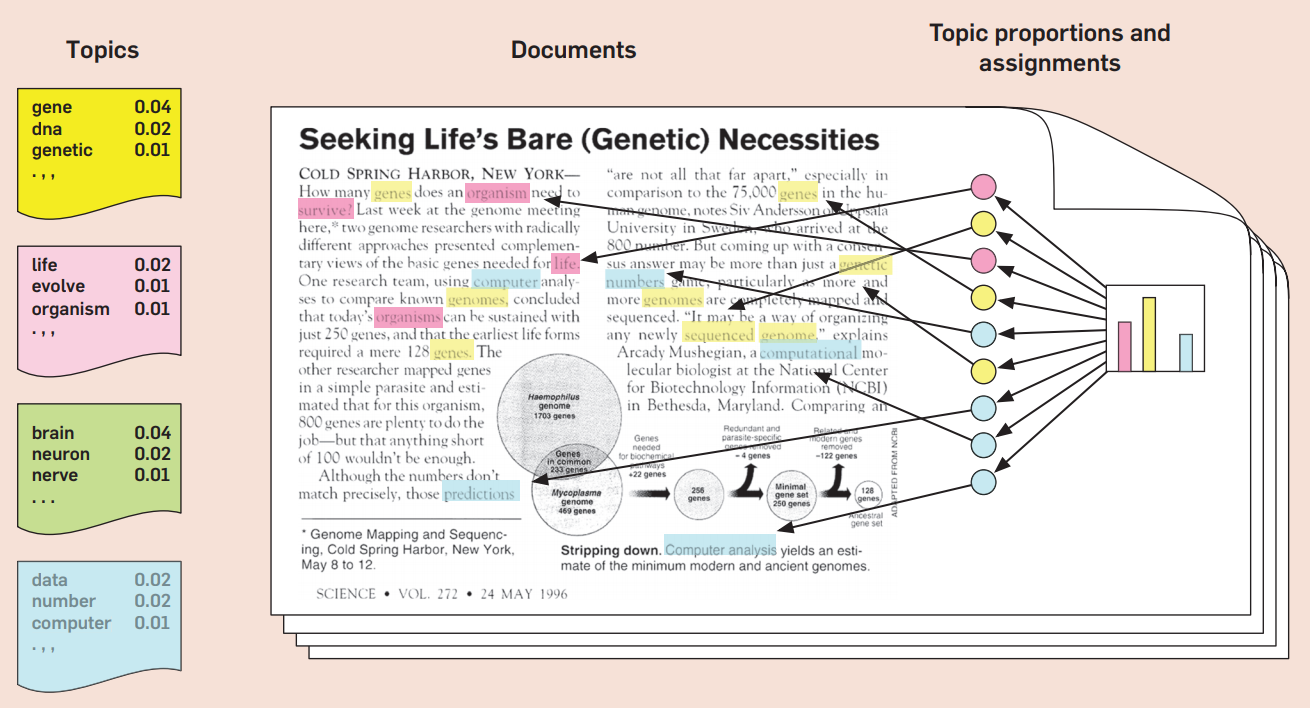
\includegraphics[width=0.8\textwidth]{document/images/lda_topic_model.png}
    % Der Teil in eckigen Klammern ist der Kurztitel für das Table of Contents
    \caption[Schematische Darstellung eines LDA Topic Modelings]{Schematische Darstellung eines LDA Topic Modelings. Quelle: \citetitle{blei_2012} \parencite{blei_2012}}
    \label{fig:lda_example}
\end{figure}

% Wenn wir nicht wollen, dass ein Kapitel auf einer neuen Seite startet, nutzen wir das hier:
{\let\clearpage\relax \chapter{Theoriefindung}}

\Blindtext

%% Bibliography

\setstretch{1.0}
\printbibliography[title={Literaturverzeichnis}]

\end{document}